
\begin{figure}
\centering
\begin{subfigure}[t]{0.32\textwidth}
\centering
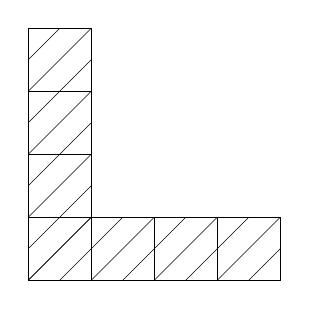
\begin{tikzpicture}[scale = 0.8]

\draw (0,0) -- (0,4) -- (1,4) -- (1,0) -- (0,0);
\foreach \a in {1,2,3} {\draw (0,\a) -- (1,\a);}
\foreach \a in {0,0.5,1,1.5,2,2.5,3} {\draw [very thin] (0,\a) -- (1,1+\a);}
\draw [very thin] (0,3.5) -- (0.5,4);
\draw (0,0) -- (4,0) -- (4,1) -- (0,1) -- (0,0);
\foreach \a in {1,2,3} {\draw (\a,0) -- (\a,1);}
\foreach \a in {0,0.5,1,1.5,2,2.5,3} {\draw [very thin] (\a,0) -- (1+\a,1);}
\draw [very thin] (3.5,0) -- (4,0.5);

\end{tikzpicture}
\caption{west: bounceback, south: bounceback}
\end{subfigure}
\begin{subfigure}[t]{0.32\textwidth}
\centering
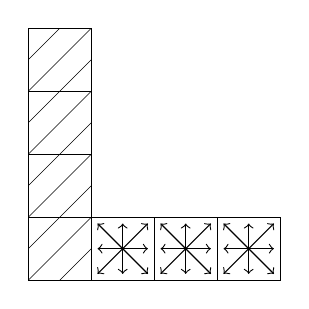
\begin{tikzpicture}[scale = 0.8]

\draw (0,0) -- (0,4) -- (1,4) -- (1,0) -- (0,0);
\foreach \a in {1,2,3} {\draw (0,\a) -- (1,\a);}
\foreach \a in {0,0.5,1,1.5,2,2.5,3} {\draw [very thin] (0,\a) -- (1,1+\a);}
\draw [very thin] (0,3.5) -- (0.5,4);
\draw [very thin] (0.5,0) -- (1,0.5);
\draw (0,0) -- (4,0) -- (4,1) -- (0,1) -- (0,0);
\foreach \a in {1,2,3} {\draw (\a,0) -- (\a,1);}
\foreach \a in {1,2,3} {\draw[->] (\a+0.5,0.5) -- (\a+0.1,0.9);}
\foreach \a in {1,2,3} {\draw[->] (\a+0.5,0.5) -- (\a+0.5,0.9);}
\foreach \a in {1,2,3} {\draw[->] (\a+0.5,0.5) -- (\a+0.9,0.9);}
\foreach \a in {1,2,3} {\draw[->] (\a+0.5,0.5) -- (\a+0.9,0.5);}
\foreach \a in {1,2,3} {\draw[->] (\a+0.5,0.5) -- (\a+0.1,0.5);}
\foreach \a in {1,2,3} {\draw[->] (\a+0.5,0.5) -- (\a+0.5,0.1);}
\foreach \a in {1,2,3} {\draw[->] (\a+0.5,0.5) -- (\a+0.1,0.1);}
\foreach \a in {1,2,3} {\draw[->] (\a+0.5,0.5) -- (\a+0.9,0.1);}

\end{tikzpicture}
\caption{west: bounceback, south: periodic}
\end{subfigure}
\begin{subfigure}[t]{0.32\textwidth}
\centering
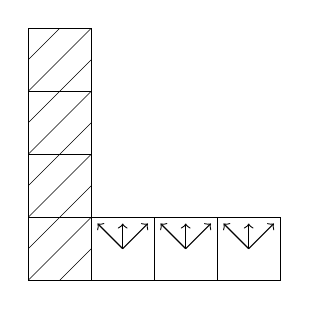
\begin{tikzpicture}[scale = 0.8]

\draw (0,0) -- (0,4) -- (1,4) -- (1,0) -- (0,0);
\foreach \a in {1,2,3} {\draw (0,\a) -- (1,\a);}
\foreach \a in {0,0.5,1,1.5,2,2.5,3} {\draw [very thin] (0,\a) -- (1,1+\a);}
\draw [very thin] (0,3.5) -- (0.5,4);
\draw [very thin] (0.5,0) -- (1,0.5);
\draw (0,0) -- (4,0) -- (4,1) -- (0,1) -- (0,0);
\foreach \a in {1,2,3} {\draw (\a,0) -- (\a,1);}
\foreach \a in {1,2,3} {\draw[->] (\a+0.5,0.5) -- (\a+0.1,0.9);}
\foreach \a in {1,2,3} {\draw[->] (\a+0.5,0.5) -- (\a+0.5,0.9);}
\foreach \a in {1,2,3} {\draw[->] (\a+0.5,0.5) -- (\a+0.9,0.9);}

\end{tikzpicture}
\caption{west: bounceback, south: pressure}
\end{subfigure}

\begin{subfigure}[t]{0.32\textwidth}
\centering
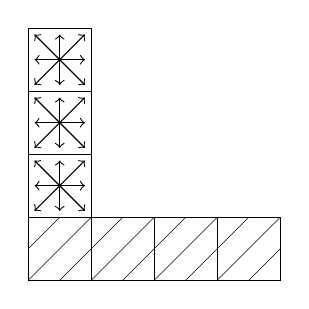
\begin{tikzpicture}[scale = 0.8]

\draw (0,0) -- (0,4) -- (1,4) -- (1,0) -- (0,0);
\foreach \a in {1,2,3} {\draw (0,\a) -- (1,\a);}
\foreach \a in {1,2,3} {\draw[->] (0.5,\a+0.5) -- (0.9,\a+0.1);}
\foreach \a in {1,2,3} {\draw[->] (0.5,\a+0.5) -- (0.9,\a+0.5);}
\foreach \a in {1,2,3} {\draw[->] (0.5,\a+0.5) -- (0.9,\a+0.9);}
\foreach \a in {1,2,3} {\draw[->] (0.5,\a+0.5) -- (0.5,\a+0.9);}
\foreach \a in {1,2,3} {\draw[->] (0.5,\a+0.5) -- (0.5,\a+0.1);}
\foreach \a in {1,2,3} {\draw[->] (0.5,\a+0.5) -- (0.1,\a+0.5);}
\foreach \a in {1,2,3} {\draw[->] (0.5,\a+0.5) -- (0.1,\a+0.1);}
\foreach \a in {1,2,3} {\draw[->] (0.5,\a+0.5) -- (0.1,\a+0.9);}
\draw (0,0) -- (4,0) -- (4,1) -- (0,1) -- (0,0);
\foreach \a in {1,2,3} {\draw (\a,0) -- (\a,1);}
\foreach \a in {0,0.5,1,1.5,2,2.5,3} {\draw [very thin] (\a,0) -- (1+\a,1);}
\draw [very thin] (3.5,0) -- (4,0.5);
\draw [very thin] (0,0.5) -- (0.5,1);

\end{tikzpicture}
\caption{west: periodic, south: bouncback}
\end{subfigure}
\begin{subfigure}[t]{0.32\textwidth}
\centering
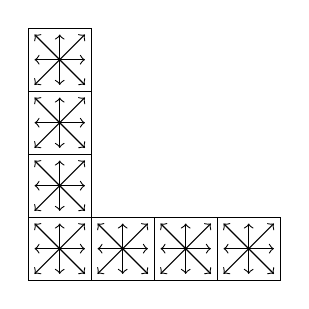
\begin{tikzpicture}[scale = 0.8]

\draw (0,0) -- (0,4) -- (1,4) -- (1,0) -- (0,0);
\foreach \a in {1,2,3} {\draw (0,\a) -- (1,\a);}
\foreach \a in {1,2,3} {\draw[->] (0.5,\a+0.5) -- (0.9,\a+0.1);}
\foreach \a in {1,2,3} {\draw[->] (0.5,\a+0.5) -- (0.9,\a+0.5);}
\foreach \a in {1,2,3} {\draw[->] (0.5,\a+0.5) -- (0.9,\a+0.9);}
\foreach \a in {1,2,3} {\draw[->] (0.5,\a+0.5) -- (0.5,\a+0.9);}
\foreach \a in {1,2,3} {\draw[->] (0.5,\a+0.5) -- (0.5,\a+0.1);}
\foreach \a in {1,2,3} {\draw[->] (0.5,\a+0.5) -- (0.1,\a+0.5);}
\foreach \a in {1,2,3} {\draw[->] (0.5,\a+0.5) -- (0.1,\a+0.1);}
\foreach \a in {1,2,3} {\draw[->] (0.5,\a+0.5) -- (0.1,\a+0.9);}
\draw (0,0) -- (4,0) -- (4,1) -- (0,1) -- (0,0);
\foreach \a in {1,2,3} {\draw (\a,0) -- (\a,1);}
\foreach \a in {0,1,2,3} {\draw[->] (\a+0.5,0.5) -- (\a+0.1,0.9);}
\foreach \a in {0,1,2,3} {\draw[->] (\a+0.5,0.5) -- (\a+0.5,0.9);}
\foreach \a in {0,1,2,3} {\draw[->] (\a+0.5,0.5) -- (\a+0.9,0.9);}
\foreach \a in {0,1,2,3} {\draw[->] (\a+0.5,0.5) -- (\a+0.9,0.5);}
\foreach \a in {0,1,2,3} {\draw[->] (\a+0.5,0.5) -- (\a+0.1,0.5);}
\foreach \a in {0,1,2,3} {\draw[->] (\a+0.5,0.5) -- (\a+0.5,0.1);}
\foreach \a in {0,1,2,3} {\draw[->] (\a+0.5,0.5) -- (\a+0.1,0.1);}
\foreach \a in {0,1,2,3} {\draw[->] (\a+0.5,0.5) -- (\a+0.9,0.1);}

\end{tikzpicture}
\caption{west: periodic, south: periodic}
\end{subfigure}
\begin{subfigure}[t]{0.32\textwidth}
\centering
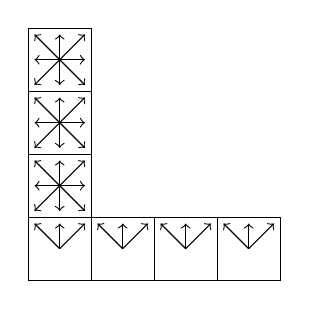
\begin{tikzpicture}[scale = 0.8]

\draw (0,0) -- (0,4) -- (1,4) -- (1,0) -- (0,0);
\foreach \a in {1,2,3} {\draw (0,\a) -- (1,\a);}
\foreach \a in {1,2,3} {\draw[->] (0.5,\a+0.5) -- (0.9,\a+0.1);}
\foreach \a in {1,2,3} {\draw[->] (0.5,\a+0.5) -- (0.9,\a+0.5);}
\foreach \a in {1,2,3} {\draw[->] (0.5,\a+0.5) -- (0.9,\a+0.9);}
\foreach \a in {1,2,3} {\draw[->] (0.5,\a+0.5) -- (0.5,\a+0.9);}
\foreach \a in {1,2,3} {\draw[->] (0.5,\a+0.5) -- (0.5,\a+0.1);}
\foreach \a in {1,2,3} {\draw[->] (0.5,\a+0.5) -- (0.1,\a+0.5);}
\foreach \a in {1,2,3} {\draw[->] (0.5,\a+0.5) -- (0.1,\a+0.1);}
\foreach \a in {1,2,3} {\draw[->] (0.5,\a+0.5) -- (0.1,\a+0.9);}
\draw (0,0) -- (4,0) -- (4,1) -- (0,1) -- (0,0);
\foreach \a in {1,2,3} {\draw (\a,0) -- (\a,1);}
\foreach \a in {0,1,2,3} {\draw[->] (\a+0.5,0.5) -- (\a+0.1,0.9);}
\foreach \a in {0,1,2,3} {\draw[->] (\a+0.5,0.5) -- (\a+0.5,0.9);}
\foreach \a in {0,1,2,3} {\draw[->] (\a+0.5,0.5) -- (\a+0.9,0.9);}

\end{tikzpicture}
\caption{west: periodic, south: pressure}
\end{subfigure}

\begin{subfigure}[t]{0.32\textwidth}
\centering
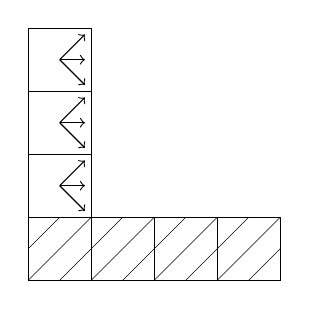
\begin{tikzpicture}[scale = 0.8]

\draw (0,0) -- (0,4) -- (1,4) -- (1,0) -- (0,0);
\foreach \a in {1,2,3} {\draw (0,\a) -- (1,\a);}
\foreach \a in {1,2,3} {\draw[->] (0.5,\a+0.5) -- (0.9,\a+0.1);}
\foreach \a in {1,2,3} {\draw[->] (0.5,\a+0.5) -- (0.9,\a+0.5);}
\foreach \a in {1,2,3} {\draw[->] (0.5,\a+0.5) -- (0.9,\a+0.9);}
\draw (0,0) -- (4,0) -- (4,1) -- (0,1) -- (0,0);
\foreach \a in {1,2,3} {\draw (\a,0) -- (\a,1);}
\foreach \a in {0,0.5,1,1.5,2,2.5,3} {\draw [very thin] (\a,0) -- (1+\a,1);}
\draw [very thin] (3.5,0) -- (4,0.5);
\draw [very thin] (0,0.5) -- (0.5,1);

\end{tikzpicture}
\caption{west: pressure, south: bounceback}
\end{subfigure}
\begin{subfigure}[t]{0.32\textwidth}
\centering
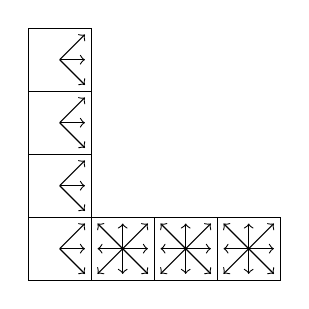
\begin{tikzpicture}[scale = 0.8]

\draw (0,0) -- (0,4) -- (1,4) -- (1,0) -- (0,0);
\foreach \a in {1,2,3} {\draw (0,\a) -- (1,\a);}
\foreach \a in {0,1,2,3} {\draw[->] (0.5,\a+0.5) -- (0.9,\a+0.1);}
\foreach \a in {0,1,2,3} {\draw[->] (0.5,\a+0.5) -- (0.9,\a+0.5);}
\foreach \a in {0,1,2,3} {\draw[->] (0.5,\a+0.5) -- (0.9,\a+0.9);}
\draw (0,0) -- (4,0) -- (4,1) -- (0,1) -- (0,0);
\foreach \a in {1,2,3} {\draw (\a,0) -- (\a,1);}
\foreach \a in {1,2,3} {\draw (\a,0) -- (\a,1);}
\foreach \a in {1,2,3} {\draw[->] (\a+0.5,0.5) -- (\a+0.1,0.9);}
\foreach \a in {1,2,3} {\draw[->] (\a+0.5,0.5) -- (\a+0.5,0.9);}
\foreach \a in {1,2,3} {\draw[->] (\a+0.5,0.5) -- (\a+0.9,0.9);}
\foreach \a in {1,2,3} {\draw[->] (\a+0.5,0.5) -- (\a+0.9,0.5);}
\foreach \a in {1,2,3} {\draw[->] (\a+0.5,0.5) -- (\a+0.1,0.5);}
\foreach \a in {1,2,3} {\draw[->] (\a+0.5,0.5) -- (\a+0.5,0.1);}
\foreach \a in {1,2,3} {\draw[->] (\a+0.5,0.5) -- (\a+0.1,0.1);}
\foreach \a in {1,2,3} {\draw[->] (\a+0.5,0.5) -- (\a+0.9,0.1);}

\end{tikzpicture}
\caption{west: pressure, south: periodic}
\end{subfigure}
\begin{subfigure}[t]{0.32\textwidth}
\centering
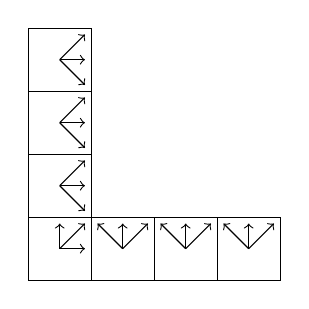
\begin{tikzpicture}[scale = 0.8]
\draw (0,0) -- (0,4) -- (1,4) -- (1,0) -- (0,0);
\foreach \a in {1,2,3} {\draw (0,\a) -- (1,\a);}

\foreach \a in {1,2,3} {\draw[->] (0.5,\a+0.5) -- (0.9,\a+0.1);}
\foreach \a in {1,2,3} {\draw[->] (0.5,\a+0.5) -- (0.9,\a+0.5);}
\foreach \a in {1,2,3} {\draw[->] (0.5,\a+0.5) -- (0.9,\a+0.9);}

\draw (0,0) -- (4,0) -- (4,1) -- (0,1) -- (0,0);
\foreach \a in {1,2,3} {\draw (\a,0) -- (\a,1);}
\foreach \a in {1,2,3} {\draw (\a,0) -- (\a,1);}

\foreach \a in {1,2,3} {\draw[->] (\a+0.5,0.5) -- (\a+0.1,0.9);}
\foreach \a in {0,1,2,3} {\draw[->] (\a+0.5,0.5) -- (\a+0.5,0.9);}
\foreach \a in {0,1,2,3} {\draw[->] (\a+0.5,0.5) -- (\a+0.9,0.9);}
\draw [->] (0.5,0.5) -- (0.9,0.5); 

\end{tikzpicture}
\caption{west: pressure, south: pressure}
\end{subfigure}
\end{figure}